\section{Phoenix的详细分析}
这一小节的将详细的分析Phoenix存在的不足,并分析造成这些不足的根本原因。

\subsection{Phoenix的内部实现}
多核下的MapReduce模型中,
Map阶段产生的key-value,都存放于一个共享的中间结构,
之前的很多研究都显示,
影响多核MapReduce系统性能的关键因素是
对该中间结构的操作效率\cite{mao2010metis}。
Phoenix的中间结构是一个全局的二维数组
(如图\ref{phoenix:intermediate}),
因此,多个map worker可以同时向其中添加数据,而多个reduce worker也可以同时从中读取数据。
为了避免多个map worker和reduce worker同时读写共享的中间结构,导致多线程间的竞争带来的数据不一致性,
Phoenix采用两种策略减少竞争:
\begin{figure}[!h!t]  
	\centering
	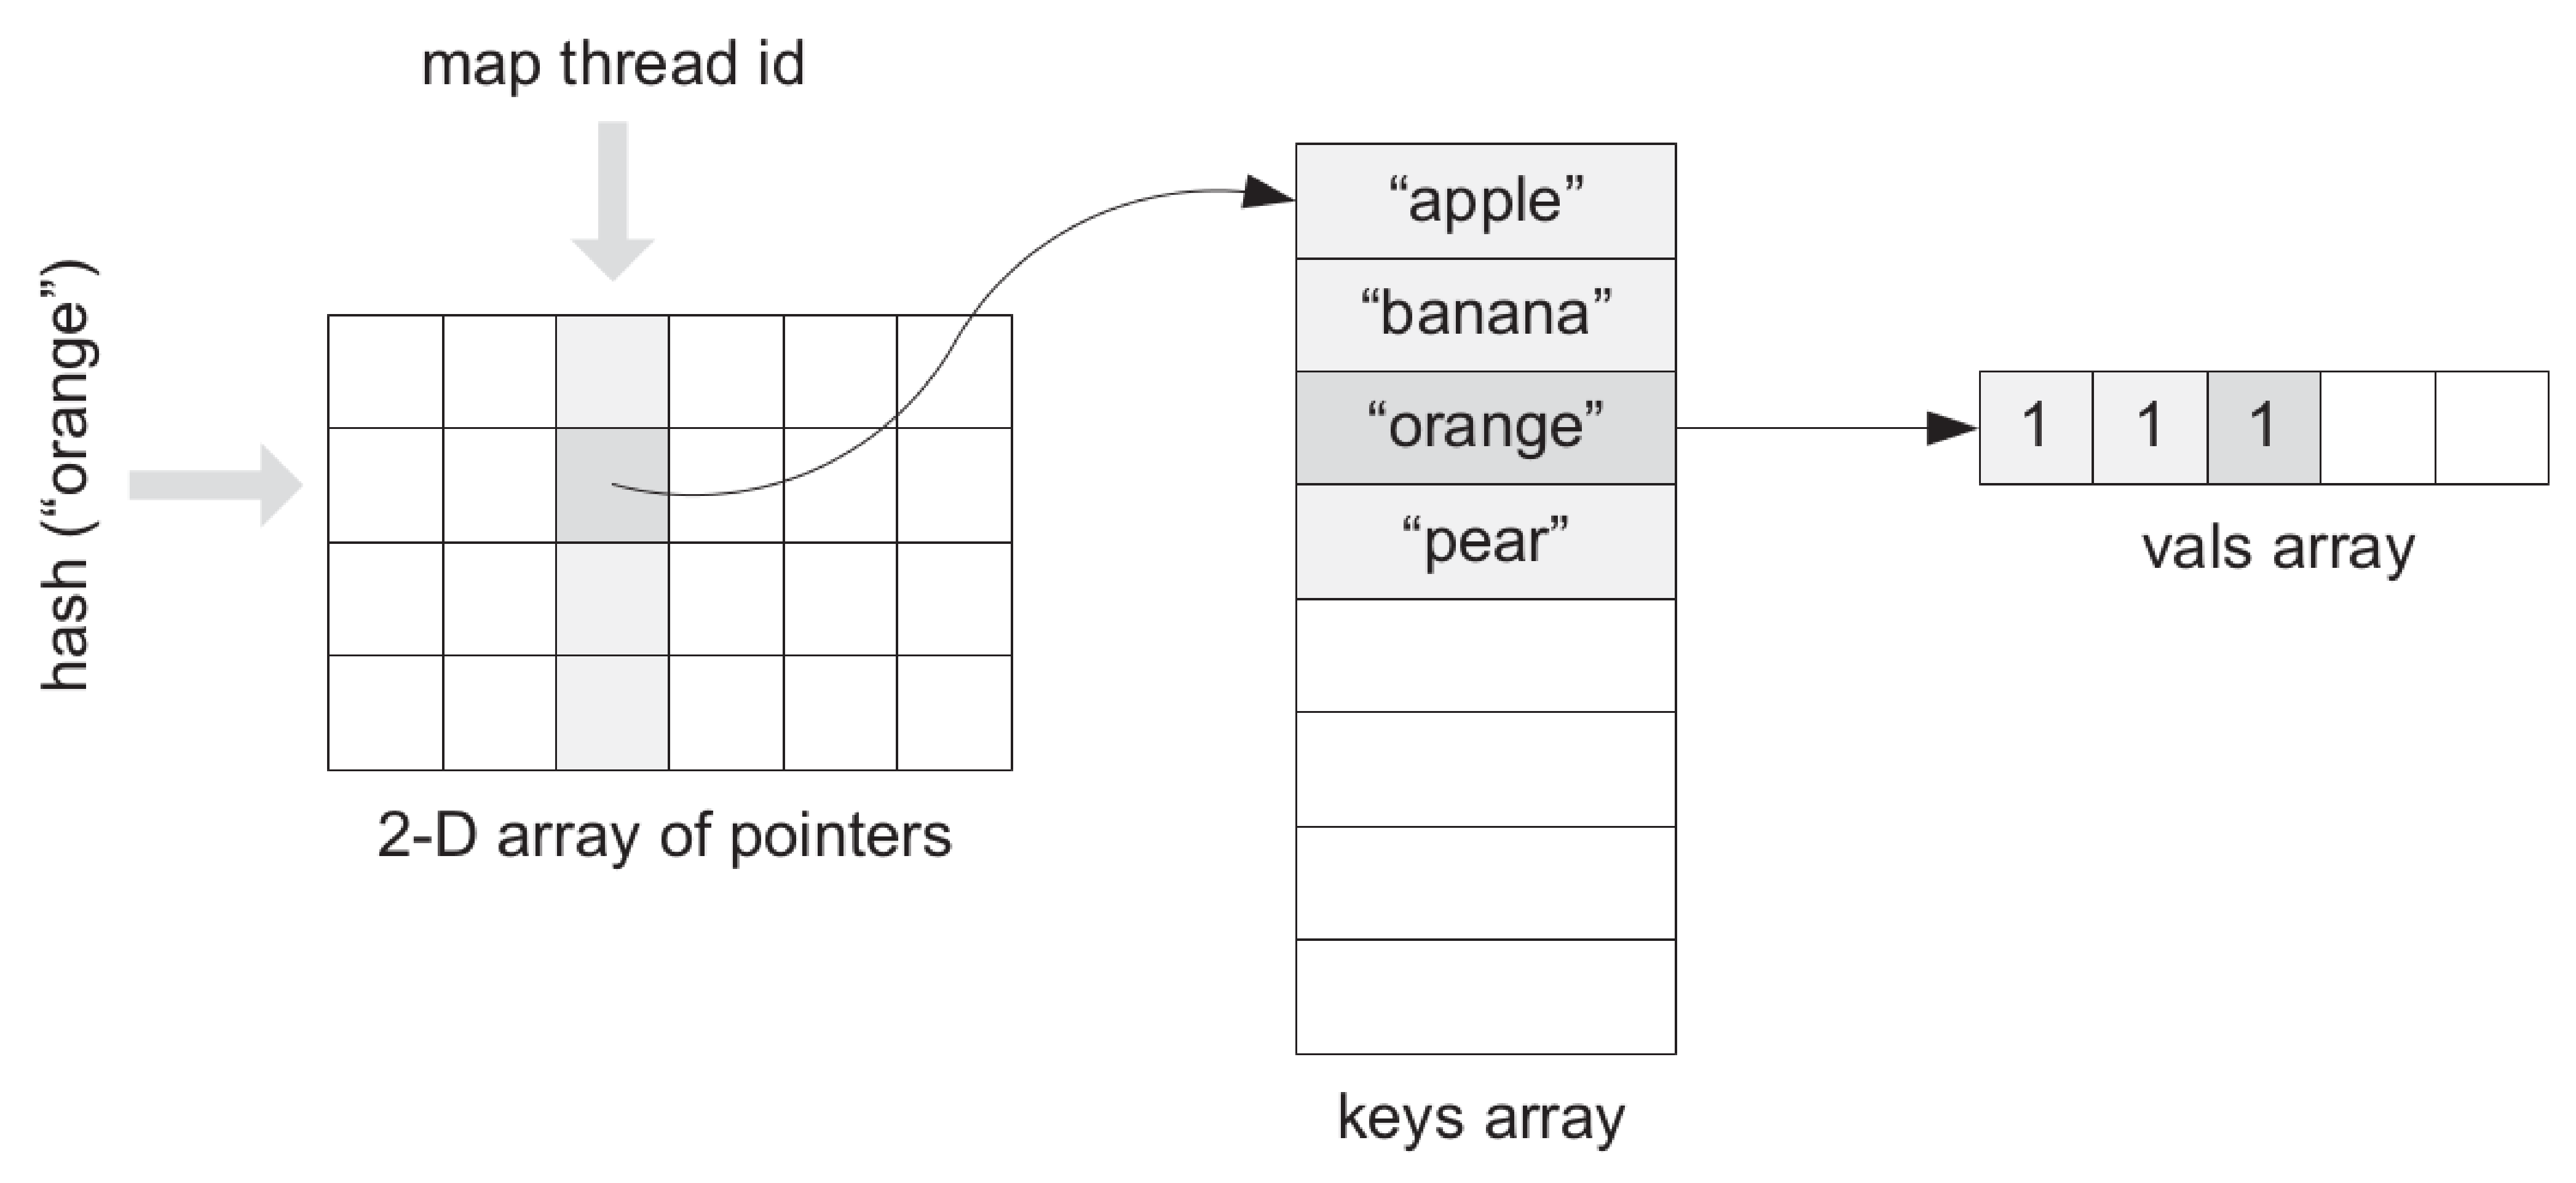
\includegraphics[width=0.75\textwidth]{img/phoenix_intermediate.eps}
	\caption{phoenix intermediate is a gobal array}
	\label{phoenix:intermediate}
\end{figure}

\begin{itemize}
	\item 对全局的二维数组进行划分:
	每个map对应二维数据的每一行,每个reduce对应每一列,
	即map和reduce都拥有自己独立的读写区域。
	可有效避免多个map或多个reduce之间读写同一区域的竞争。
	
	\item 为了避免map和reduce的交织,
	Phoenix在map和reduce之间加入屏障barrier,
	即Map阶段结束后,才能开始Reduce阶段。
	从而可以避免map和reduce对同一区域的竞争。
	
\end{itemize}
通过采用以上两种策略,可以有效减少应用程序中锁的使用,
从而简化程序,\grayt{如实验结果显示pthread\_mutex和pthread\_cond的开销相当小。} %测试Phoenix中的mutex和cond的时间,给出数据。
但是这些策略却限制了Phoenix的性能,接下来的章节中将会详细的解释。

\subsection{scalability的缺陷}
Phoenix中存在大量的堆对象的操作,因此Phoenix的性能和scalability受到内存分配器的影响。
glibc中自带的内存分配器ptmalloc对多核的可伸缩性较差\cite{gloger1997ptmalloc},
相比之下,jemalloc\cite{evans2006jemalloc}具有较好的可伸缩性。
为了对比两种分配器对性能的影响,我们将Phoenix分别与ptmalloc和jemalloc进行编译,
记为Phoenix-jemalloc和Phoenix-ptmalloc,
并将应用程序在不同分配器下的运行时间进行对比。
通过对比实验,结果如图\ref{fig:phoenix:jemalloc:ptmalloc}所示,
对大部分应用程序,在核数较高的情况下,
Phoenix-jemalloc比Phoenix-ptmalloc具有更好的性能。

\begin{figure}[!h!t]
	\centering
	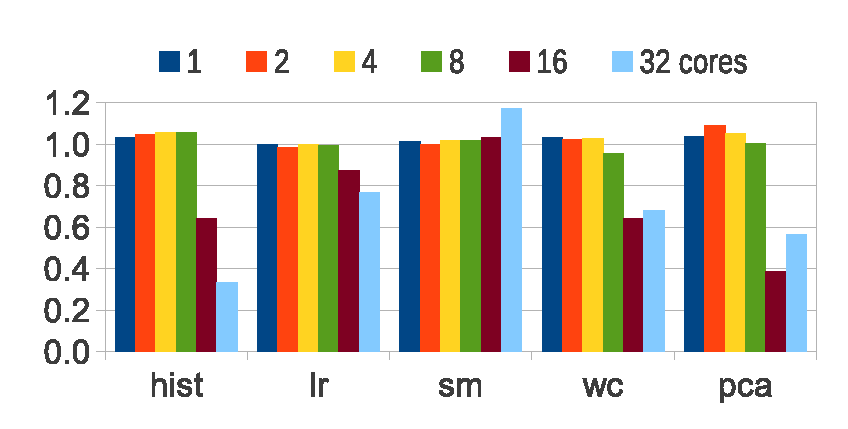
\includegraphics[width=0.5\textwidth]{eps/phoenix_jemalloc_ptmalloc.eps}
	\caption{Execution time of Phoenix-jemalloc to Phoenix-ptmalloc}
	\label{fig:phoenix:jemalloc:ptmalloc}
\end{figure}

图\ref{fig:phoenix:speedup}展示的是Phoenix-ptmalloc的speedup。
从图中我们可以看出,随着核数的增多,性能越来越差。
这里我们将查看Phoenix使用性能较好的内存分配器jemalloc后,
各应用程序的speedup,实验结果如图\ref{fig:phoenix:speedup:jemalloc}所示。
从图中可以看出,从1到8核情况下,随着核数的增多,
各个应用程序的性能越来越好。但是,当核数操作8核时,
wc和hist的性能越来越差;当核数超过16核时,lr, sm和pca的性能越来越差。
从实验的结果我们可以得出,即使使用性能较好的jemalloc内存分配器,
Phoenix的scalability也相当的差,当核数超过16时,
基于Phoenix-jemalloc的应用程序的性能都会变差。

\begin{figure}[!h!t]
	\centering
	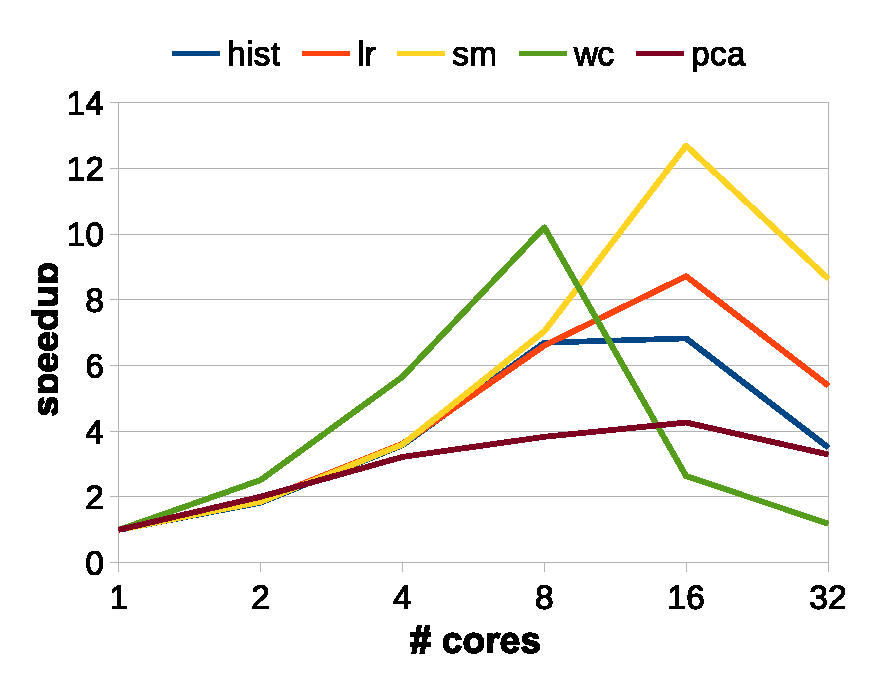
\includegraphics[width=0.5\textwidth]{eps/phoenix_speedup_jemalloc.eps}
	\caption{Speedup of Phoenix-jemalloc}
	\label{fig:phoenix:speedup:jemalloc}
\end{figure}

为了分析Phoenix较差的scalability,我们使用Linux Perf\cite{de2009performance}
收集热点函数的执行时间信息。
结果显示,在核数较低的情况下,map函数占用整个运行时间的比例最大,
但是当增加更多核数时(即超过8核时),\lock 函数将成为最热的函数。
\lock 是Linux内核中的一种典型自旋锁,用于保护共享数据结构。
锁的开销反映了Linux内核中的竞争情况,为了更加清楚分析这种自旋锁\lock 对应用程序的影响,
我们测试各个应用程序在不同核数情况下的竞争情况。

如图\ref{fig:phoenix:spinlock}给出了各个应用程序分别在Phoenix-ptmalloc和Phoenix-jemalloc情况下,
\lock 占用的时间比例。
从实验结果中可以看出,当核数超过8时,\lock 的开销占用将迅速上升。
具体地,对于hist在16和32核情况下,\lock 占用的总运行时间的比例分别为39.6\%和51.61\%。
实验结果证明,基于Phoenix运行的应用程序,
当核数超过8时,将存在激烈的锁竞争。

由Linux Perf产生的函数调用栈显示,
基于Phoenx-ptmalloc的hist中,\lock 主要来源于page\_fault和mprotect系统调用,分别占用85.76\%和14.17\%。
而基于Phoenix-jemalloc的hist中,\lock 主要来源于page\_fault和mmap系统调用,分别占用89.82\%和10.18\%。
这两种不同的来源是由于不同分配器的原因。
\lock 是由于多个线程对一个唯一的读写锁mmap\_sem的竞争造成的。
接下来的章节中,我们将详细的解释,为什么多个线程需要竞争一个唯一的mmap\_sem信号量。

\begin{figure}[!h!t]  
	\centering
	\subfigure[Workloads with Phoenix-ptmalloc]{
		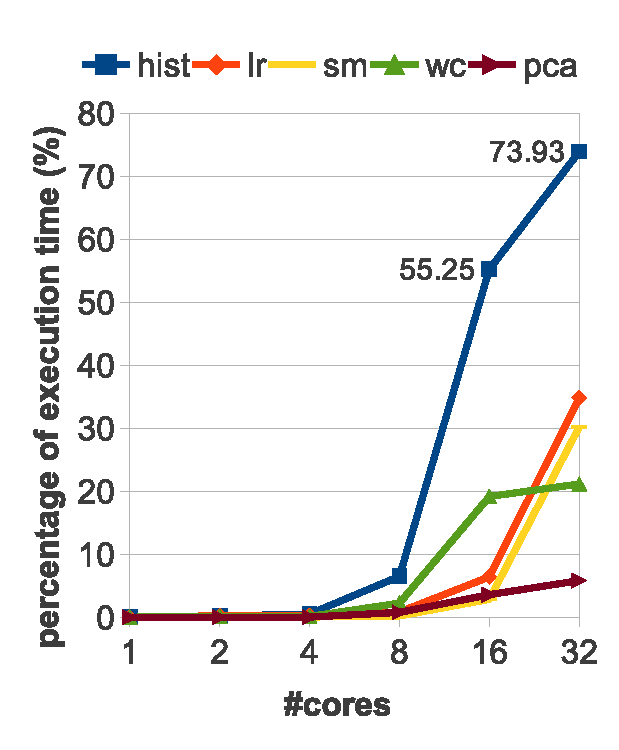
\includegraphics[width=0.21\textwidth]{eps/phoenix_spinlock_ptmalloc.eps}
		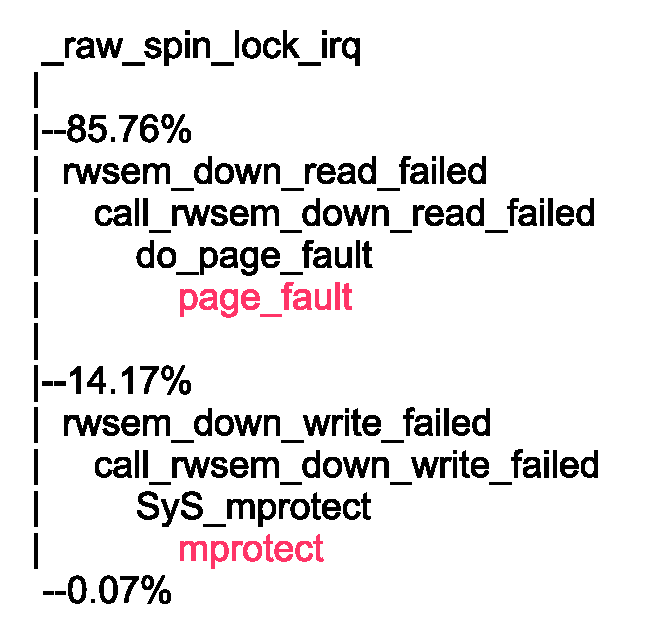
\includegraphics[width=0.26\textwidth]{eps/hist32stack_ptmalloc.eps}
		\label{fig:phoenix:spinlock:ptmalloc}
	}
	\subfigure[Workloads with Phoenix-jemalloc]{
		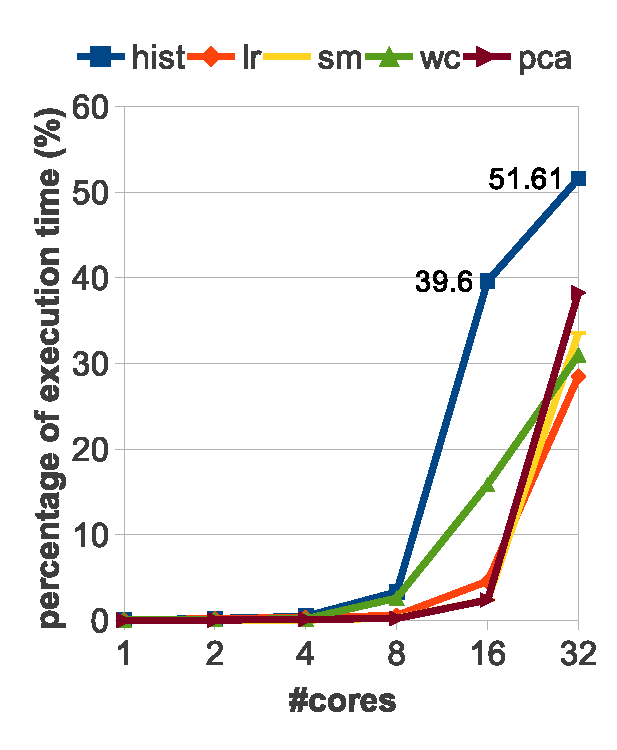
\includegraphics[width=0.22\textwidth]{eps/phoenix_spinlock_jemalloc.eps}
		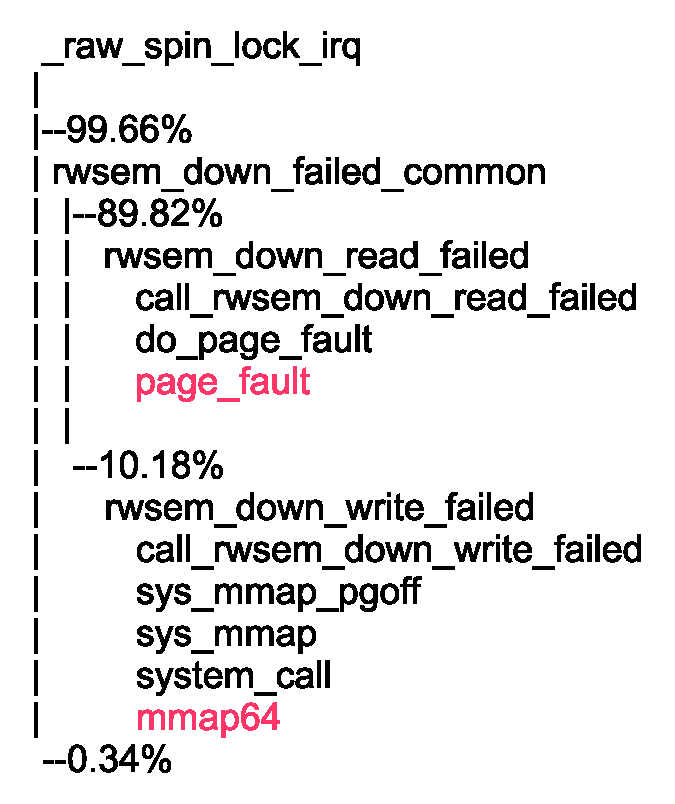
\includegraphics[width=0.25\textwidth]{eps/hist32stack_jemalloc.eps}
		\label{fig:phoenix:spinlock:jemalloc}
	}
	\caption{
		The overhead cost by \lock for
		workloads with Phoenix-ptmalloc or Phoenix-jemalloc}
	\label{fig:phoenix:spinlock}
\end{figure}



\subsection{多线程地址空间的竞争}
Phoenix利用基于共享内存的Pthreads实现并行,
基于Phoenx的应用程序中,所有的线程将共享同一进程的地址空间。
在广泛使用的操作系统中,例如Linux,
进程的地址空间通常由多个线性区(VMA)组成,
每个VMA代表一快连续的虚拟地址空间。
Linux中,进程的所有VMA通过链表链接起来,此外还会有一个红黑树来组织所有的VMA。
使用红黑树的目的是为了加快对某个特定VMA查找的速度,如图\ref{fig:mmap:sem}所示。
与红黑树对应的是一个读写信号量mmap\_sem,
当多个线程需要同时修改和查找该红黑树时,首先需要获取mmap\_sem,以保证数据的一致性。

\begin{figure}[!h!t]  
	\centering
	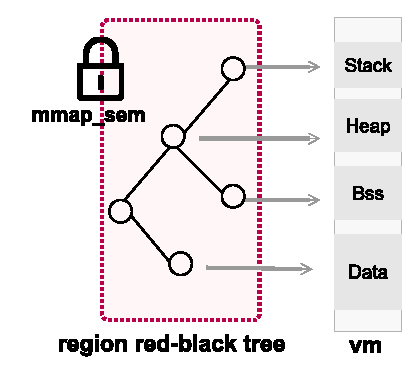
\includegraphics[width=0.40\textwidth]{eps/mmap_sem.eps}
	\caption{Address space is protected by mmap\_sem}
	\label{fig:mmap:sem}
\end{figure}


操作系统提供给用户的系统调用:\kn{mmap},\kn{munmap}和\kn{mprotect}
会修改红黑树(这些操作我们统称为内存映射操作)。
具体表现为:\kn{mmap}会创建一个新的线性区vma,并将其插入到红黑中;
\kn{munmap}会移除一块线性区,并调整红黑树;\kn{mprotect}则会修改红黑树中某个节点(vma)的访问权限域。
除了这几种更新操作外,当进程访问一个非法的虚拟地址空间时,
便会触发一个page-fault,page-fault的handler首先会查找地址空间(即查询红黑树),
确定该地址是否为合法的地址,之后再做相应的处理。
总之,多个线程共享一个进程的地址空间时,多个线程并发的产生,\kn{mmap},\kn{munmap}和\kn{mprotect},或者page-faults时,它们会并发的访问或修改同一个红黑树,
这需要内核有一定的同步手段,保证多个线程并发执行时的正确性。

为了保证进程地址空间数据的一致性,Linux使用了一个读写信号量mmap\_sem信号量,
由于同步(如图\ref{fig:mmap:sem}所示),
这是一个典型的读写信号量,它的特点是,同一时刻可以有多个读者同时持有锁,但只能有一个写着持有锁,且读者和写者不能同时获得锁。
Linux内核中,一个线程如果需要调用内存映射操作,那么它首先需要以写模式获取mmap\_sem信号量,
一旦获取后,便阻碍其他线程进行内存映射操作或page-fault的handle执行。
相应地,当发生page-fault的时候,handler函数的执行路径是,首先需要以读模式获取mmap\_sem信号量,
因此多个page-faults可以并发的执行。
通过mmap\_sem信号量,保证了地址空间数据的一致性,却让多个并发的内存映射操作和page-fault串行的执行,
这让






\subsection{Phoenix的内部实现}
多核下的MapReduce模型中,
Map阶段产生的key-value,都存放于一个共享的中间结构,
之前的很多研究都显示,
影响多核MapReduce系统性能的关键因素是
对该中间结构的操作效率\cite{mao2010metis}。
\begin{figure}[!h!t]  
    \centering
    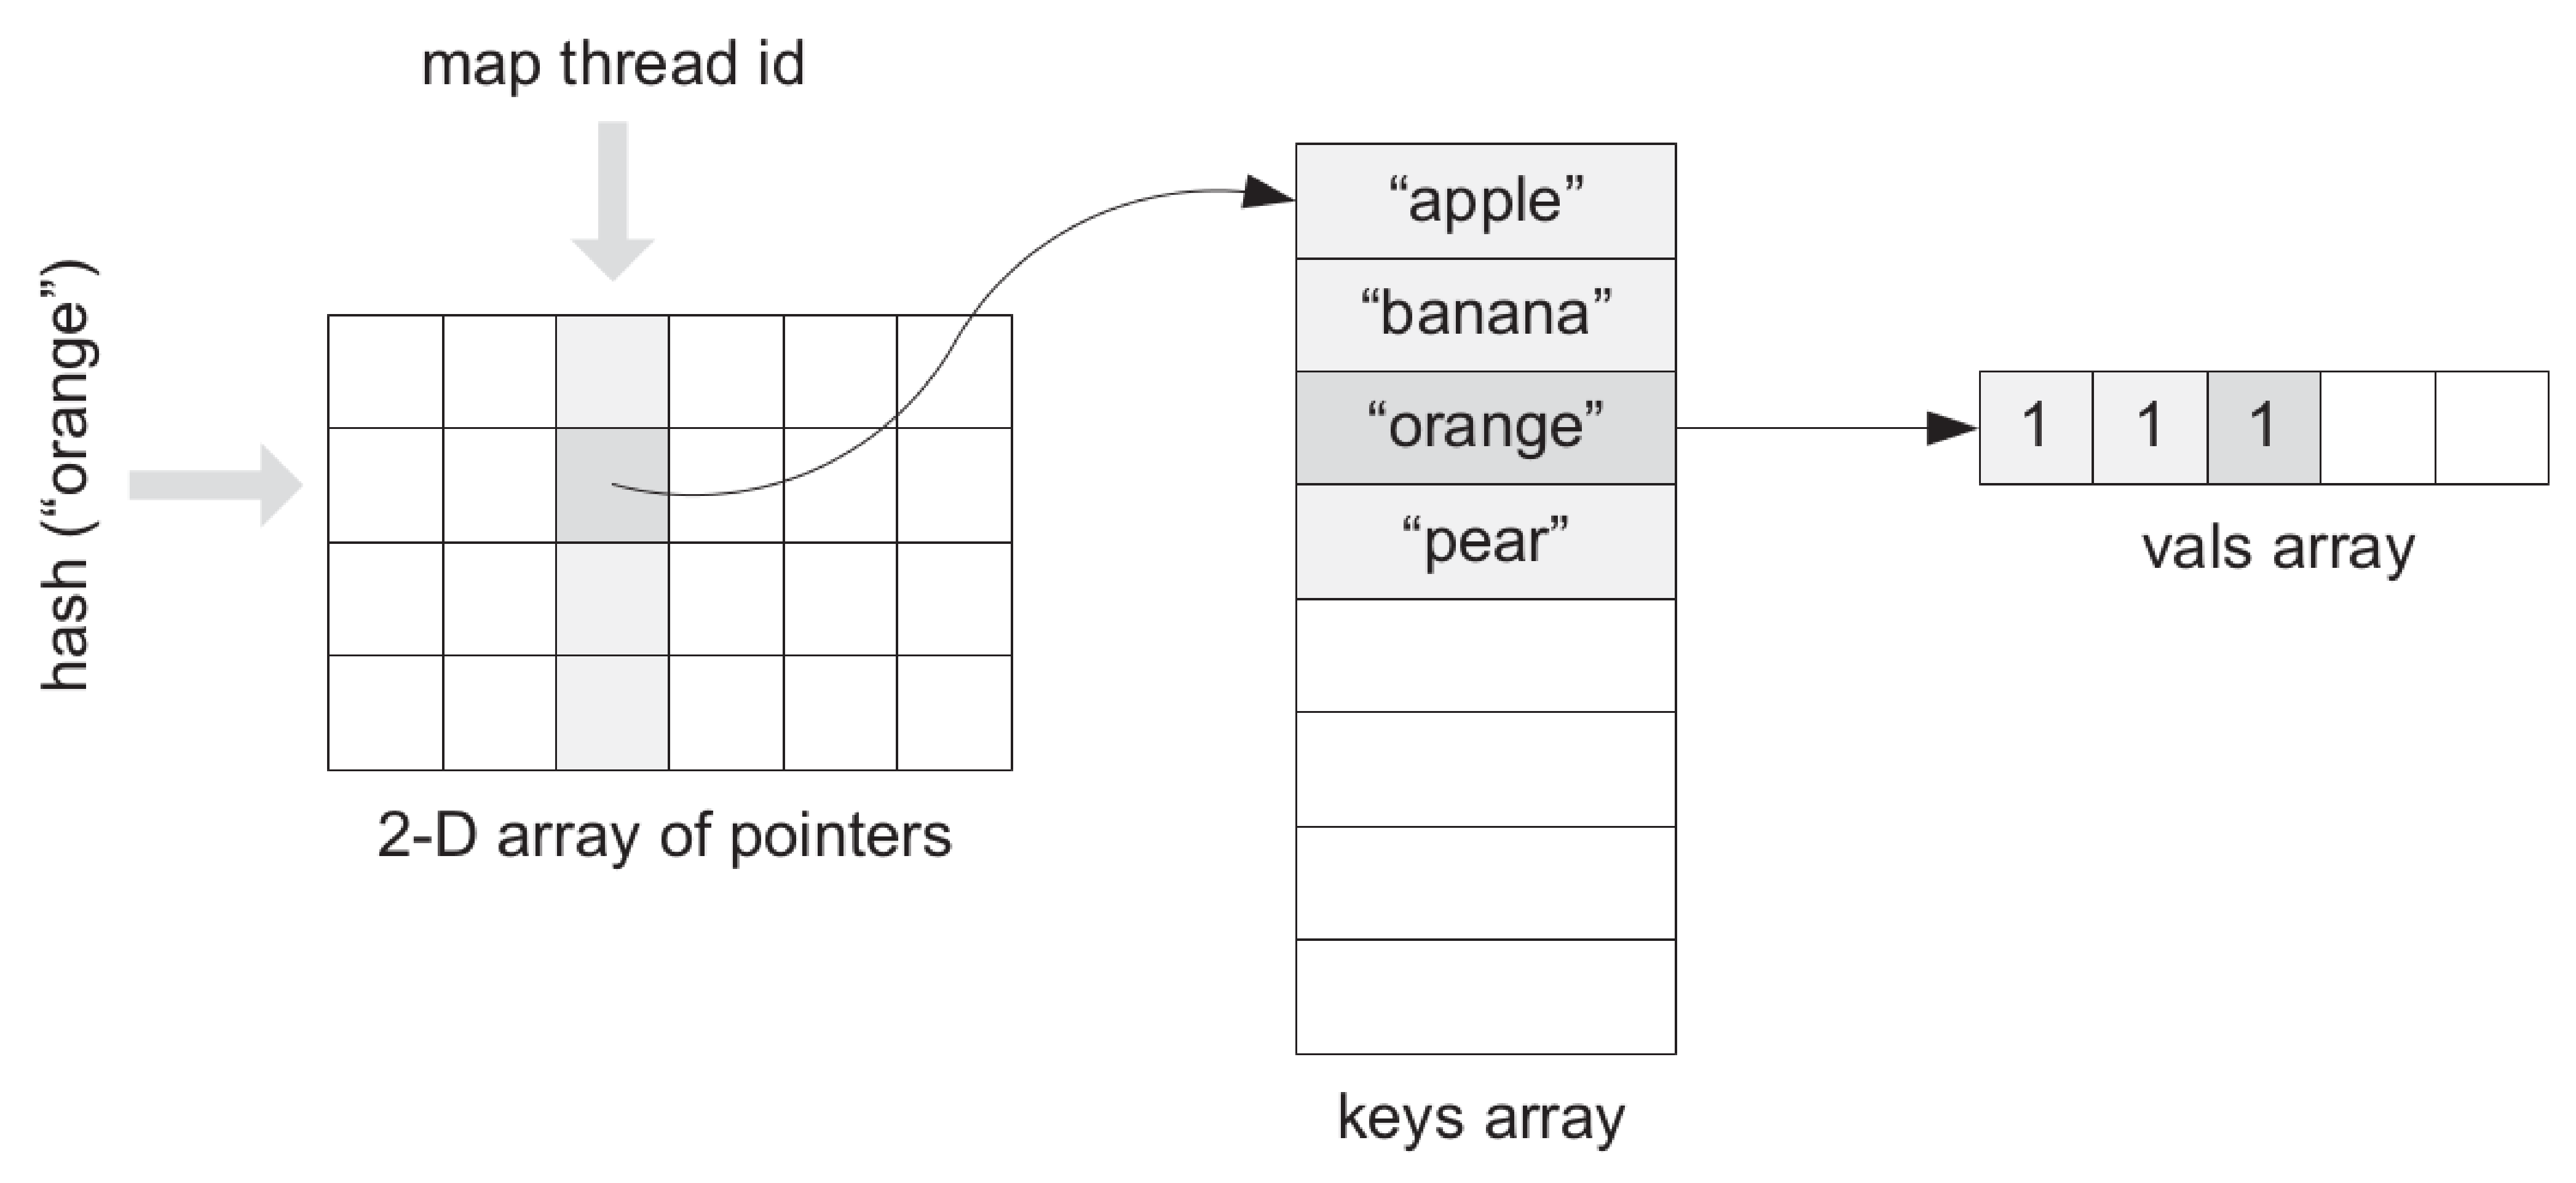
\includegraphics[width=0.75\textwidth]{img/phoenix_intermediate.eps}
    \caption{phoenix intermediate is a gobal array}
    \label{phoenix:intermediate}
\end{figure}

Phoenix中间结构是一个全局的二维数组
(如图\ref{phoenix:intermediate}),
map worker向其中增加数据,而reduce worker将读取数据,
为了避免多个map worker和reduce worker对
共享的中间结构竞争, 保证数据的一致性,
Phoenix采用两种策略:
\begin{itemize}
  \item 对全局的二维数组进行划分:
  每个map对应二维数据的每一行,每个reduce对应每一列,
  即map和reduce都拥有自己独立的读写区域。
  可有效避免多个map或多个reduce之间读写同一区域的竞争。

  \item 为了避免map和reduce的交织,
  Phoenix在map和reduce之间加入barrier,
  即Map阶段结束后,才能开始Reduce阶段。
  可以避免map和reduce对同一区域的竞争。
\end{itemize}
通过采用这两种策略,可以有效减少应用程序中锁的使用,
从而简化程序,如实验结果显示pthread\_mutex和pthread\_cond

Map阶段通常会进行大量的计算,
Reduce阶段则是需要大量的内存访问。
如果像Phoenix一样,在Map和Reduce之间加入barrier,
即等到所有的Map阶段结束,才开始reduce计算,
就会存在两个问题:
\begin{itemize}
  \item 不利于CPU的利用率,Map阶段会集中使用CPU,
  而Reduce阶段需要大量的内存访问,
  CPU资源被浪费。
  \item reduce阶段开始时间,由最慢的map worker决定;
  当某个map worker非常慢,便会影响整体的性能
\end{itemize}

DMR设计实现中,首先打破Phoenix的barrier,
不再使用共享的中间结构,DMR中的每个map worker
都拥有属于自己的私有buffer(buffer的设计细节见下一节),
一旦buffer中的key-value达到一定的阈值便发送给相应的reduce worker,
reduce收到key-value后,不等map worker结束便开始reduce工作,
即Map和Reduce阶段并发的粒度变小,
这既能充分利用资源,又能提高计算的速度。

特别地,当我们采用array buffer,
并且在map阶段不开启combiner时,
Map阶段不需要对key-value排序,即无需key的查找和插入,以及memmove等操作。
map worker产生key-value后,只需简单地将其追加到buffer中即可,
这减轻的Map阶段的工作量。key-value的排序工作由Reduce承担,
reduce worker对收到的key-value进行有序插入。
虽然整个过程的工作量并未减少,
但是Reduce的排序工作与Map阶段是并发执行的,
从而整个过程的时间变小,提高运行的效率。

此外,为了防止数据的倾斜,即大量的key-value被发送到一个reduce worker,
在Reduce阶段,我们添加了局部的reduce过程(即combiner),
一旦某个Reduce收到某个key-value的数量超过预先设定的值,
便会触发combiner,从而避免过多的内存分配带来的开销,
防止内存溢出。

DMR中map worker和reduce worker之所以能够进行流水并行执行,
是因为它们基于一个Producer-Consumer model,
在这个model中,每个map worker都拥有一个私有的buffer,
map woker是这个buffer的生产者,reduce是buffer的消费者,
当buffer中的数据达到一个阈值时,
reduce便可以取到buffer中的数据开始工作,
而不需要等到所有map结束。



虽然Phoenix为程序员提供了简单编程的手段,
它却存在一定的局限性。
\begin{figure}[!h!t]  
    \centering
    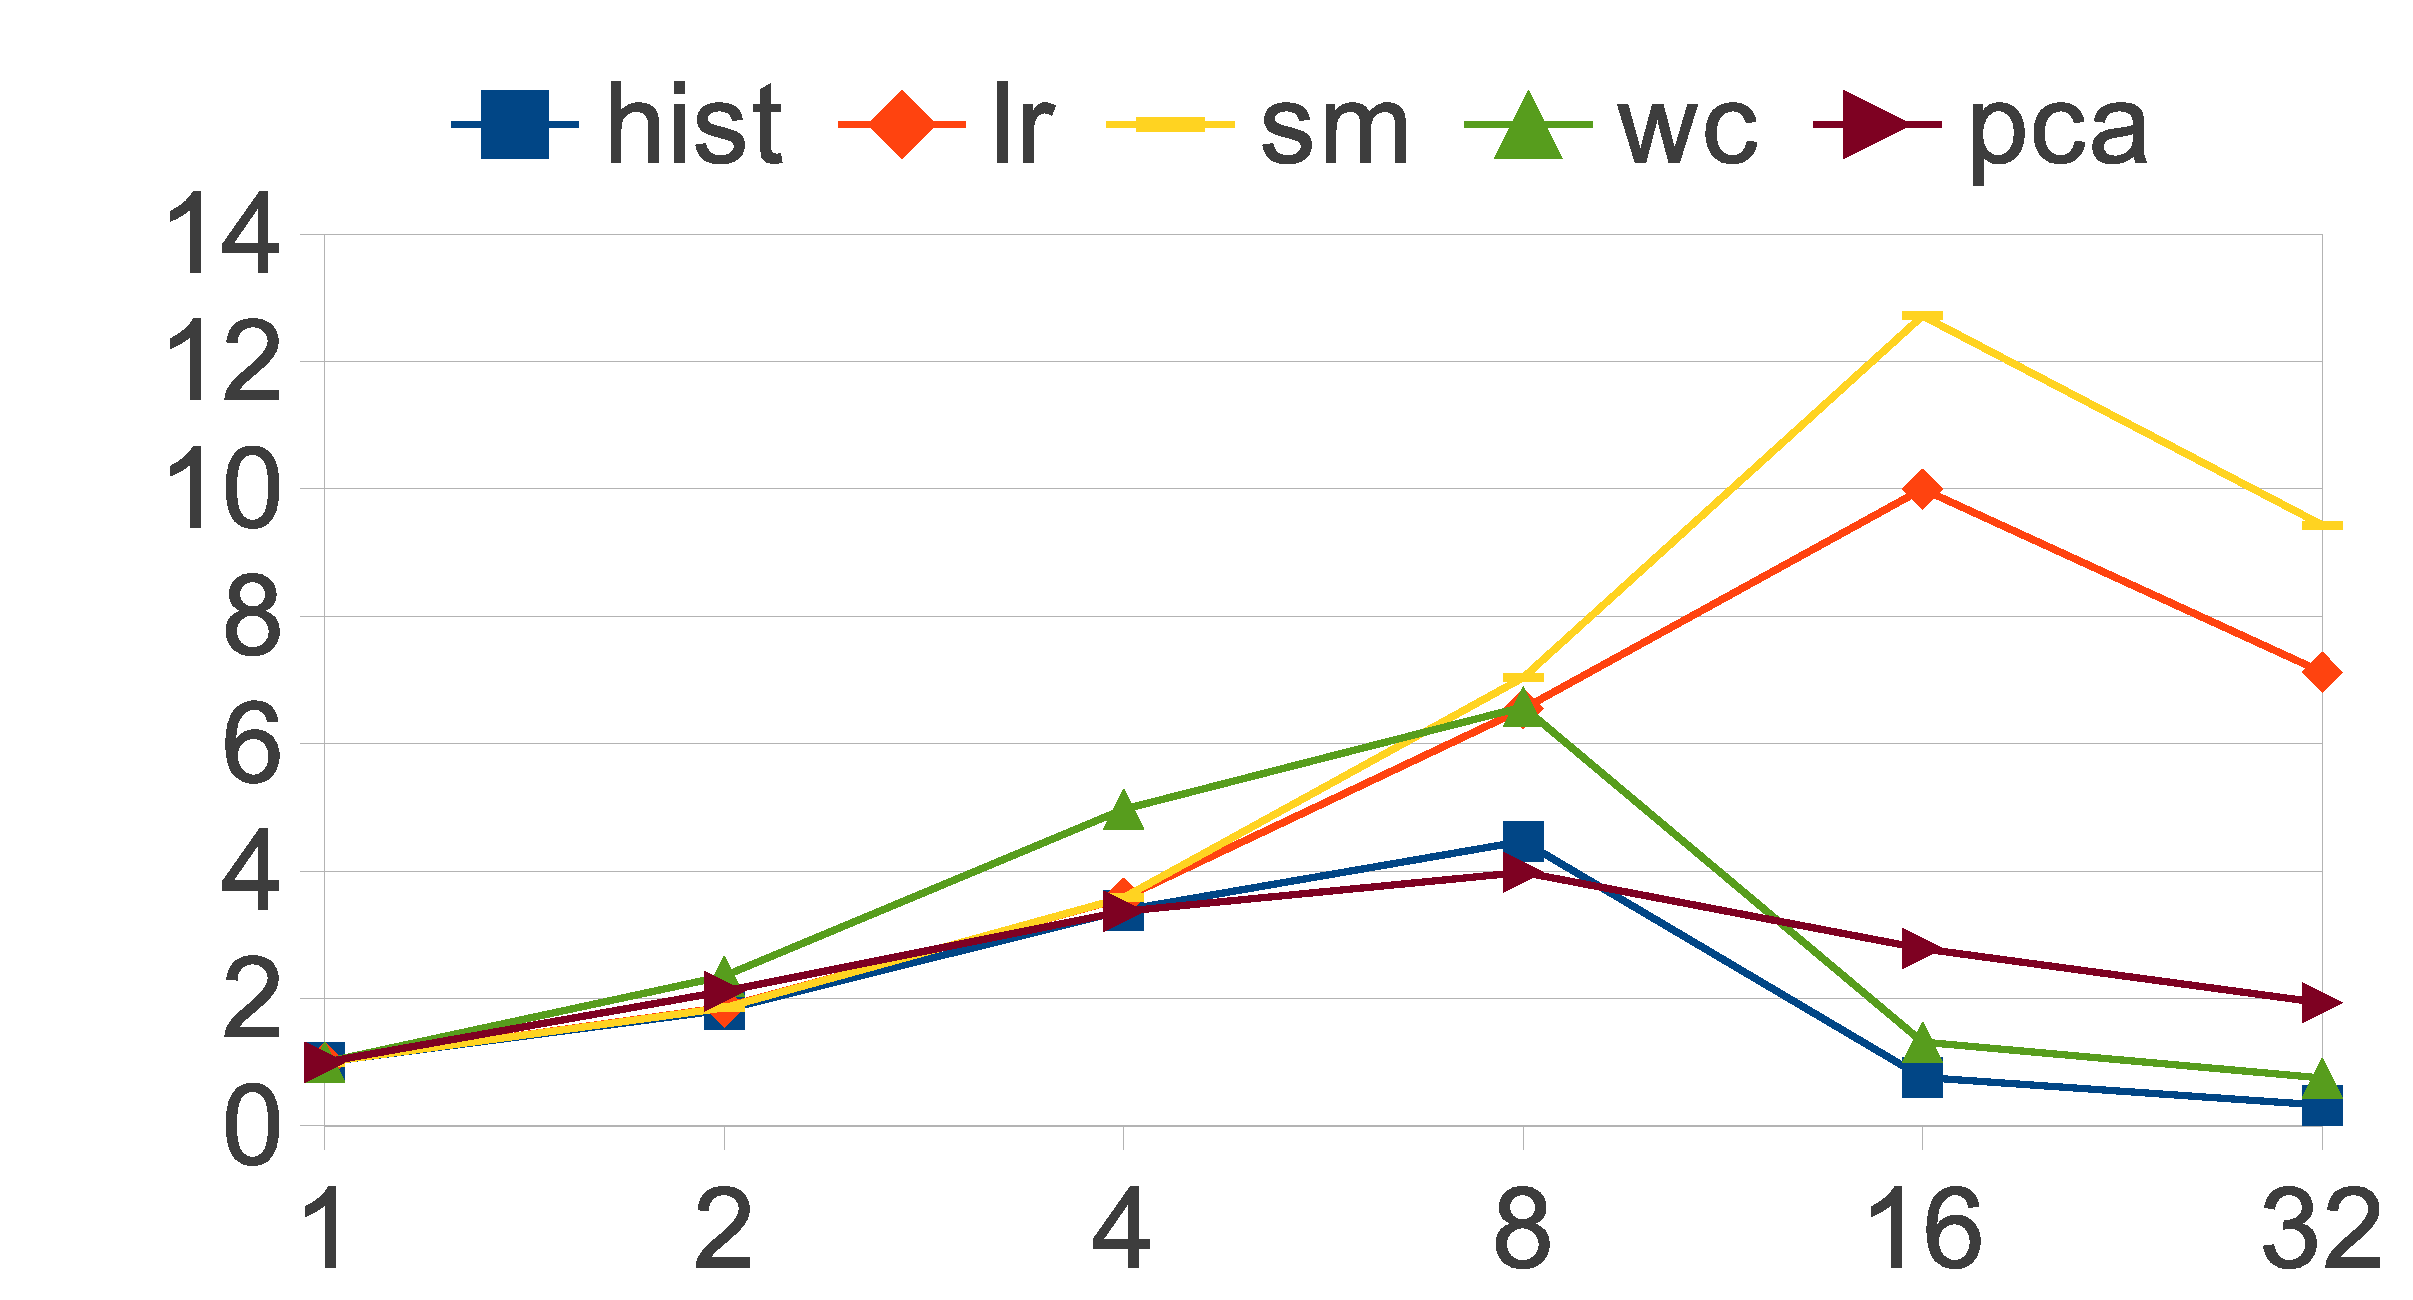
\includegraphics[width=0.5\textwidth]{img/phoenix_speedup.eps}
    \caption{Phoenix不开启Combiner情况下的Speedup}
    \label{phoenix:speedup}
\end{figure}
如图\ref{phoenix:speedup}的数据结果
(speedup计算方法为:高核下的运行时间/单核下的运行时间),
我们可以得出这样的结论:
随着核数的增多,4核以下,Phoenix的性能越来越好;
超过4核,Phoenix的性能却越来越差,特别是hist, wc, pca。

Phoenix的上述特性意味着,针对低核的机器,
它能够充分利用其资源,对于高核处理器,
Phoenix并不能充分利用资源。
Phoenix不适合在8核以上的机器上运行。
然而,多核机器是一个趋势,
一个CPU甚至达到上百的core\cite{Borkar2007Thousand},
随着多核机器上核数的不断增多,Phoenix便不具有实际的可用性。

制约Phoenix性能的主要因素有以下几点:
\begin{enumerate}
  \item Phoenix基于Posix线程库实现,开启的线程越多,
  需要共享的内核资源越多,会因为竞争这些资源
  以及共享的数据结构导致过高的spinlock.
  在32核情况下,hist的spinlock占用71.25\%。
  后续章节会详细分析Phoenix的spinlock问题。
  
  \item 由于中间结构的局限,
  Phoenix中Map阶段与Reduce阶段中间
  存在一个严格的barrier,降低了map和reduce线程
  并发的程度。此外,通常情况下,map是computation-intensivex的,
  reduce是memory-intensive的\cite{talbot2011phoenix++},
  barrier会导致资源的利用率比较低。
\end{enumerate}

DMR将针对上述的局限性进行改进和优化,
即避免Spinlock以获得较好的scalability,
同时打破原来的barrier,
增加Map和Reduce阶段并发的程度,
从而获得更好的性能。








总结:


  
